\chapter{AdS/CFT对偶}
\section{大$N$极限}
本节的主要思想在\ref{B.5}中已经介绍不少了,本节目的是把目光局限在$SU(N)$ Y-M理论,这一话题的绝佳参考资料是\href{https://www.damtp.cam.ac.uk/user/tong/gaugetheory.html}{David Tong的规范场论讲义}对应章节。
\subsection{复习规范场}
首先随便\footnote{实际上这一选取不能是随便的,需要有些限制,详见Gelis\cite{Gelis:2019yfm}。}选一个规范群$G$。然后再加入一些标量场或者旋量场,它们处于$G$的某个表示之中,也就是说,在:
\begin{equation}\label{4.1.1}
	\phi_i(x)\mapsto U_{ij}\phi_j(x),\quad U_{ij}\in G
\end{equation}
的场位形变换下$\phi_i$(略去了旋量指标)的作用量应该保持不变,理论具有$G$的内禀对称性。现在我们把$U_{ij}$换成一个local的东东,也就是把每个元素都换成一个和空间位置有关的函数。显然我们利用$\phi_i$构造的拉氏量$\mathcal{L}(\partial\phi,\phi)$不一定在local的规范群下是不变的,罪魁祸首就是$\partial$,现在还要多出$\partial U$的项。可以考虑引入一个规范场$A^\mu$,在规范群的作用下如此变换:\footnote{其实就是在说其处于自伴表示下}
\begin{equation}\label{4.1.2}
	A_\mu(x)\mapsto U(x)A_\mu (x)U^\dagger (x)+\frac i g U(x)\partial_\mu U^\dagger(x)
\end{equation}
注意这里$A_\mu$是一个$N\times N$的矩阵形式的场,我们略去了矩阵指标,它也可以在生成元$T^a$基底下展开为$A^a T^a$。如果我们做下面的替换:
\begin{equation}
	\mathcal{L}(\partial\phi,\phi)\mapsto\mathcal{L}(D\phi,\phi),\quad D_\mu\equiv \partial_\mu -igA_\mu
\end{equation}
那么可以证明$\mathcal{L}$就在local规范群的作用下也是不变的,也就是说对场位形进行变换\ref{4.1.1}和\ref{4.1.2}导致的物理是不变的,而场位形本身不是可测的,我们关心的是场的激发导致的散射振幅。这意味着场位形空间是存在冗余的,这些由规范群联系起来的场位形应该看作是同一个场,路径积分也只用积一次,这直接导致了鬼场作为一个辅助场的存在。\footnote{这里有点微妙,$\phi_i$路径积分里面还是需要积分所有场位形,因为我们应该把\ref{4.1.1}看作是规范场变换\ref{4.1.2}诱导出来的一个被动的变换,所以一旦我们通过FP量子化方法取定了$A$的一个规范,那么用$U$联系的$\phi$也要看成不同。就像是现在把$A$当成横轴,$\phi$当纵轴,把$y=kx,k\in\mathbb{R}$线上的$(A,\phi)$看成等同,为了消除冗余,可以先固定$A$,那么$\phi$依然是自由的,每个$\phi$给出一个物理上独立的场位形$(A,\phi)$。}
\begin{remark}
	说到这里还是要多说一点,global的对称性和local的规范对称性看起来都是对场操作一下后$\mathcal{L}$不变,或者差个全导数。但是前者是真正的动力学对称性,也就是说可以用Noether定理推出非平凡守恒荷的,但是后者仅仅只是数学上描述的冗余,why?因为我们讲动力学对称性,话题的主角不是场位形本身,而是场的激发产生的物理态,动力学对称性就是说对态进行变换后得到一个新的态,两者的运动方程形式完全一致,物理上可区分这两个不同的态,但是它们遵循相同的演化方程,运动方程的这种对称性就定义为动力学对称性。而local的规范对称性只是数学上的冗余,只是拉氏量本身的对称性,没有任何的动力学意义,也就是说变换前后两个态就是物理上无法区分的,而且不会带来非平凡守恒荷。所以前者我们场位形需要全积,后者我们只需要积某个特定规范下的场位形。当然,在无穷远处不归0的规范变换实际上是真正的对称性,即所谓渐近对称性,这个就不多谈了,具体可见A.Strominger的工作。
\end{remark}

\subsection{大$N$极限下的Yang-Mills理论}
规范场有两种视角来看,第一种就是因为我们要求的散射振幅是$\left<A^aA^b\cdots\right>$这些带色指标的分量场构成的关联函数(前面还要乘上对应的极化矢量)。所以可以直接用$A^a$来写费曼规则。第二种就是由于$A^a=\tr \left(A T^a\right)$,所以我们可以先把$A^\mu$就看作一个独立的矩阵,直接从矩阵来写费曼规则,最后原则上散射振幅就能用$\left<{A^{i}}_j{A^{k}}_l\ldots\right>$求迹得到。类似于\ref{B.5}中的double line表示,考虑纯的YM理论:\footnote{也完全可以考虑和费米子耦合的理论,只是需要加上单线表示费米子,加入新的顶点,稍稍复杂一些,后面再讨论。}
\begin{equation}
	S_\mathrm{YM}=-\frac1{2g^2}\int d^4x\mathrm{~tr~}F^{\mu\nu}F_{\mu\nu}
\end{equation}
为了理论的UV行为良定义,耦合常数在$N\to\infty$的过程中必须跟着变,t'Hooft定义$\lambda\equiv g^2N$,我们所说的$N\to\infty$的理论是指$\lambda$保持不变,$N\to\infty$:
\begin{equation}
	S_\mathrm{YM}=-\frac N{2\lambda}\int d^4x\mathrm{~tr~}F^{\mu\nu}F_{\mu\nu}
\end{equation}
首先计算自由胶子传播子:
\begin{equation}
	\left<A_{\mu j}^i(x)A_{\nu l}^k(y)\right>=\Delta_{\mu\nu}(x-y)\left(\delta_l^i\delta_j^k-\frac1N\delta_j^i\delta_l^k\right)\sim \Delta_{\mu\nu}(x-y)\mathrm{~}\delta_l^i\delta_j^k
\end{equation}
这一步就已经做了近似,实际上是在把$SU(N)$理论近似为$U(N)$的理论。利用double line表示,费曼图为:
\begin{figure}[H]
	\centering
	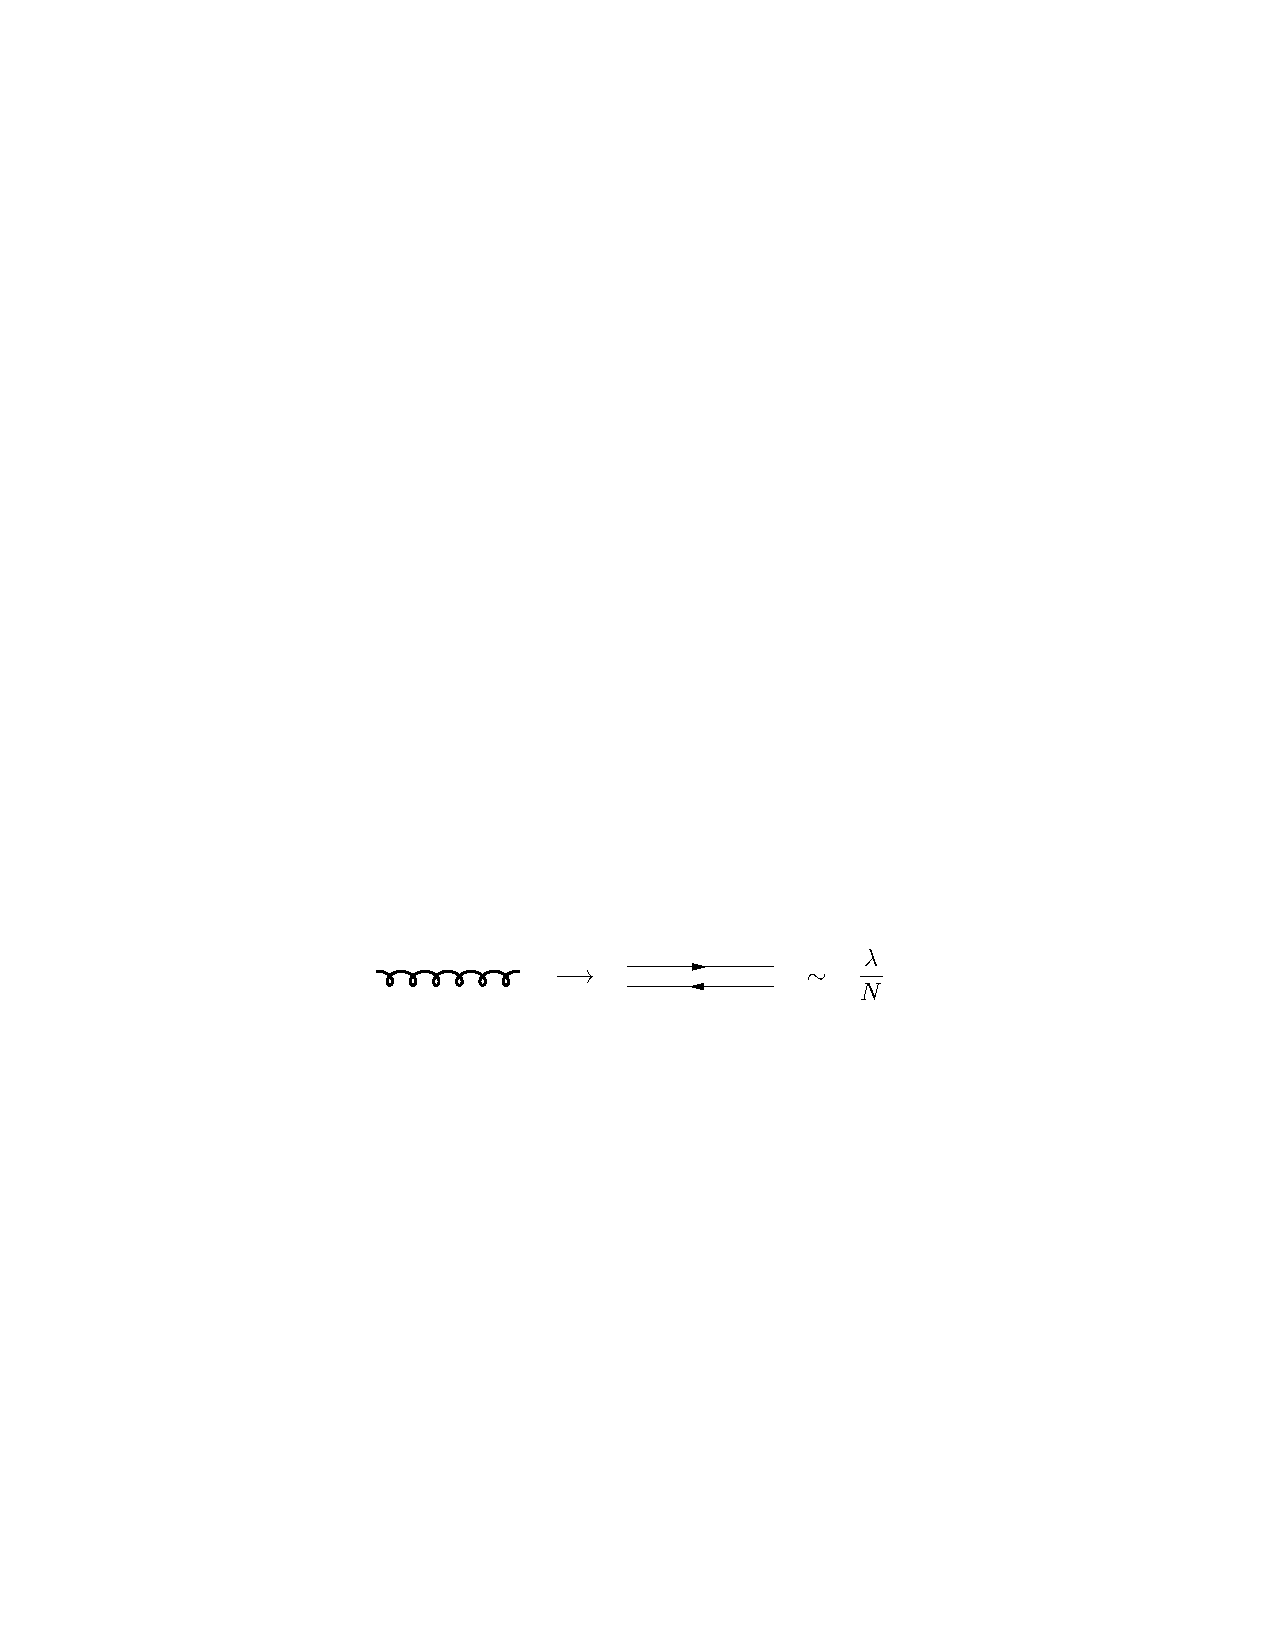
\includegraphics{figs/fig14.pdf}
\end{figure}
我们仅仅关心费曼图关于$N$的幂次,具体形式可以从色因子形式的费曼图结构看出来,后面也不会真正去计算一个double line的费曼图。这里忽略了鬼场的影响,不过就后面讨论的目的而言问题不大。另外还有下面胶子子相互作用顶点:
\begin{figure}[H]
	\centering
	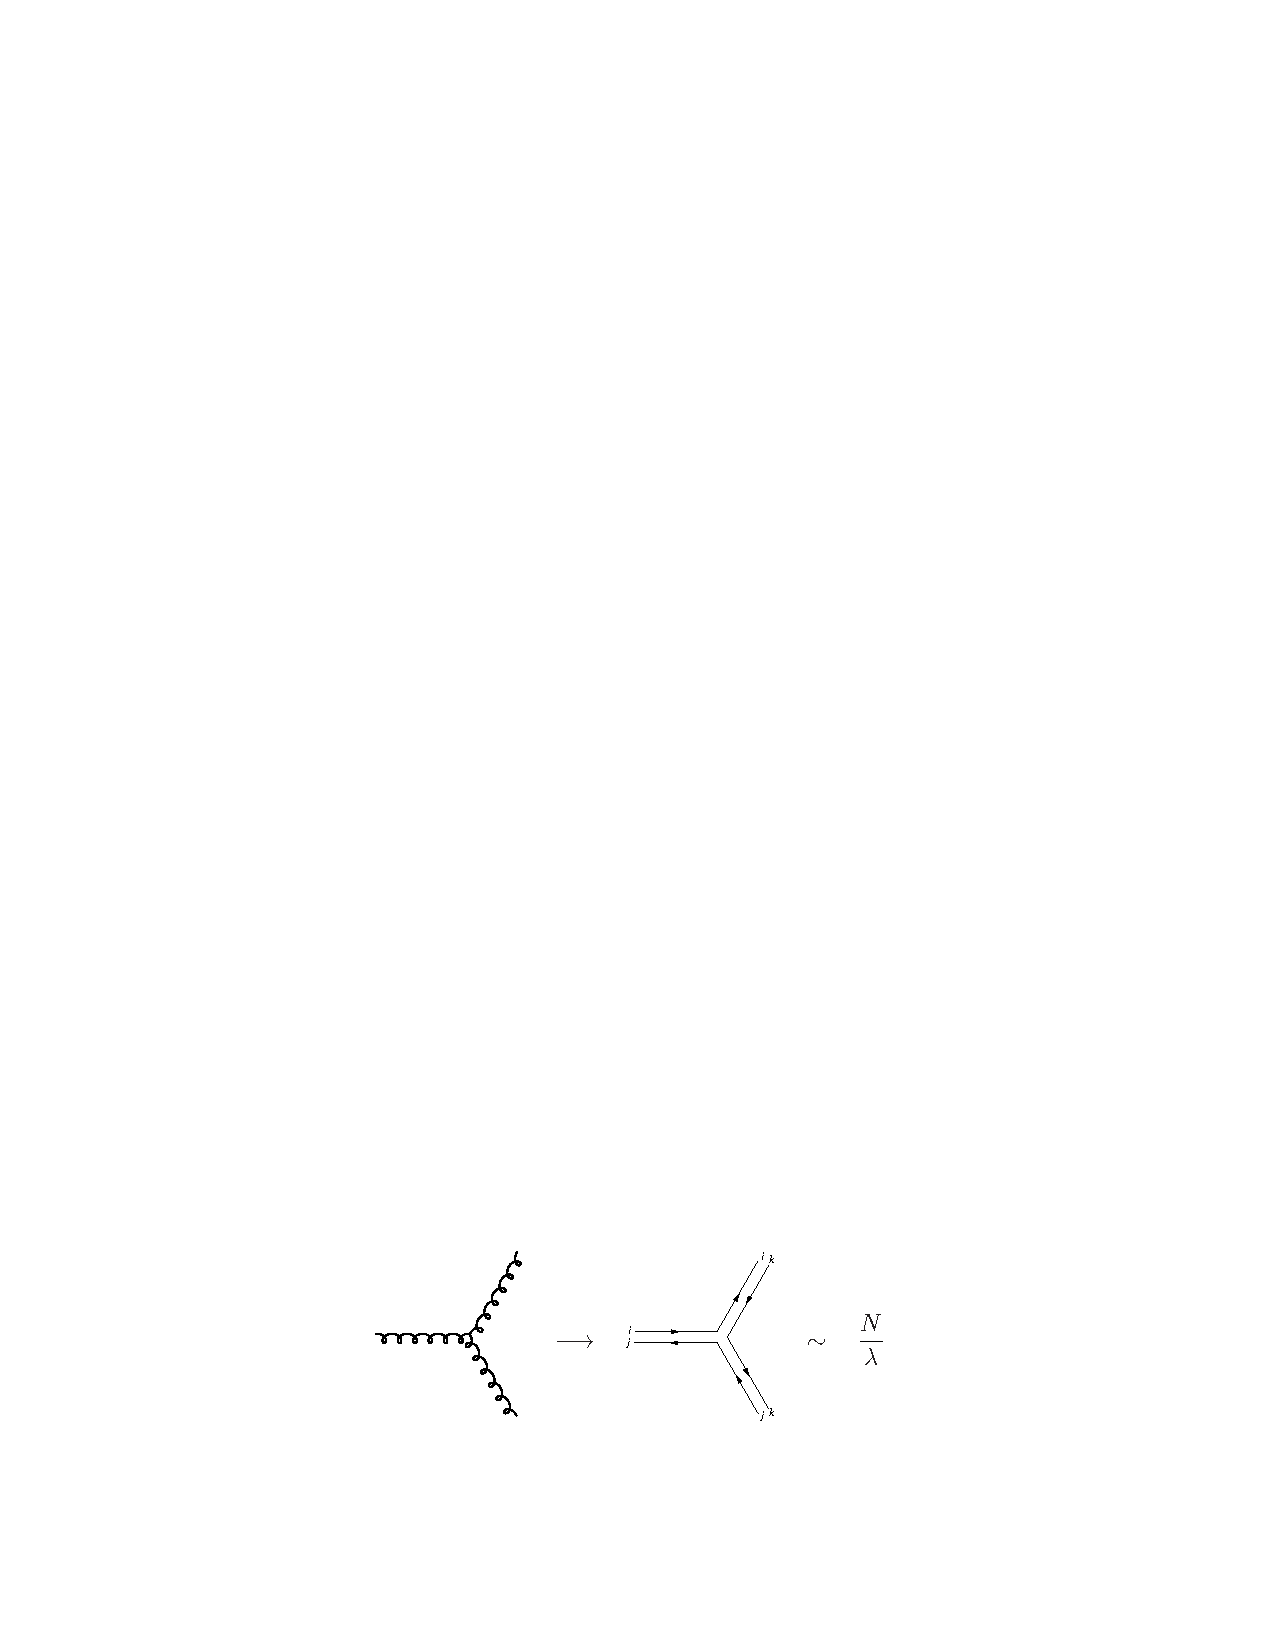
\includegraphics{figs/fig15.pdf}
\end{figure}
\begin{figure}[H]
	\centering
	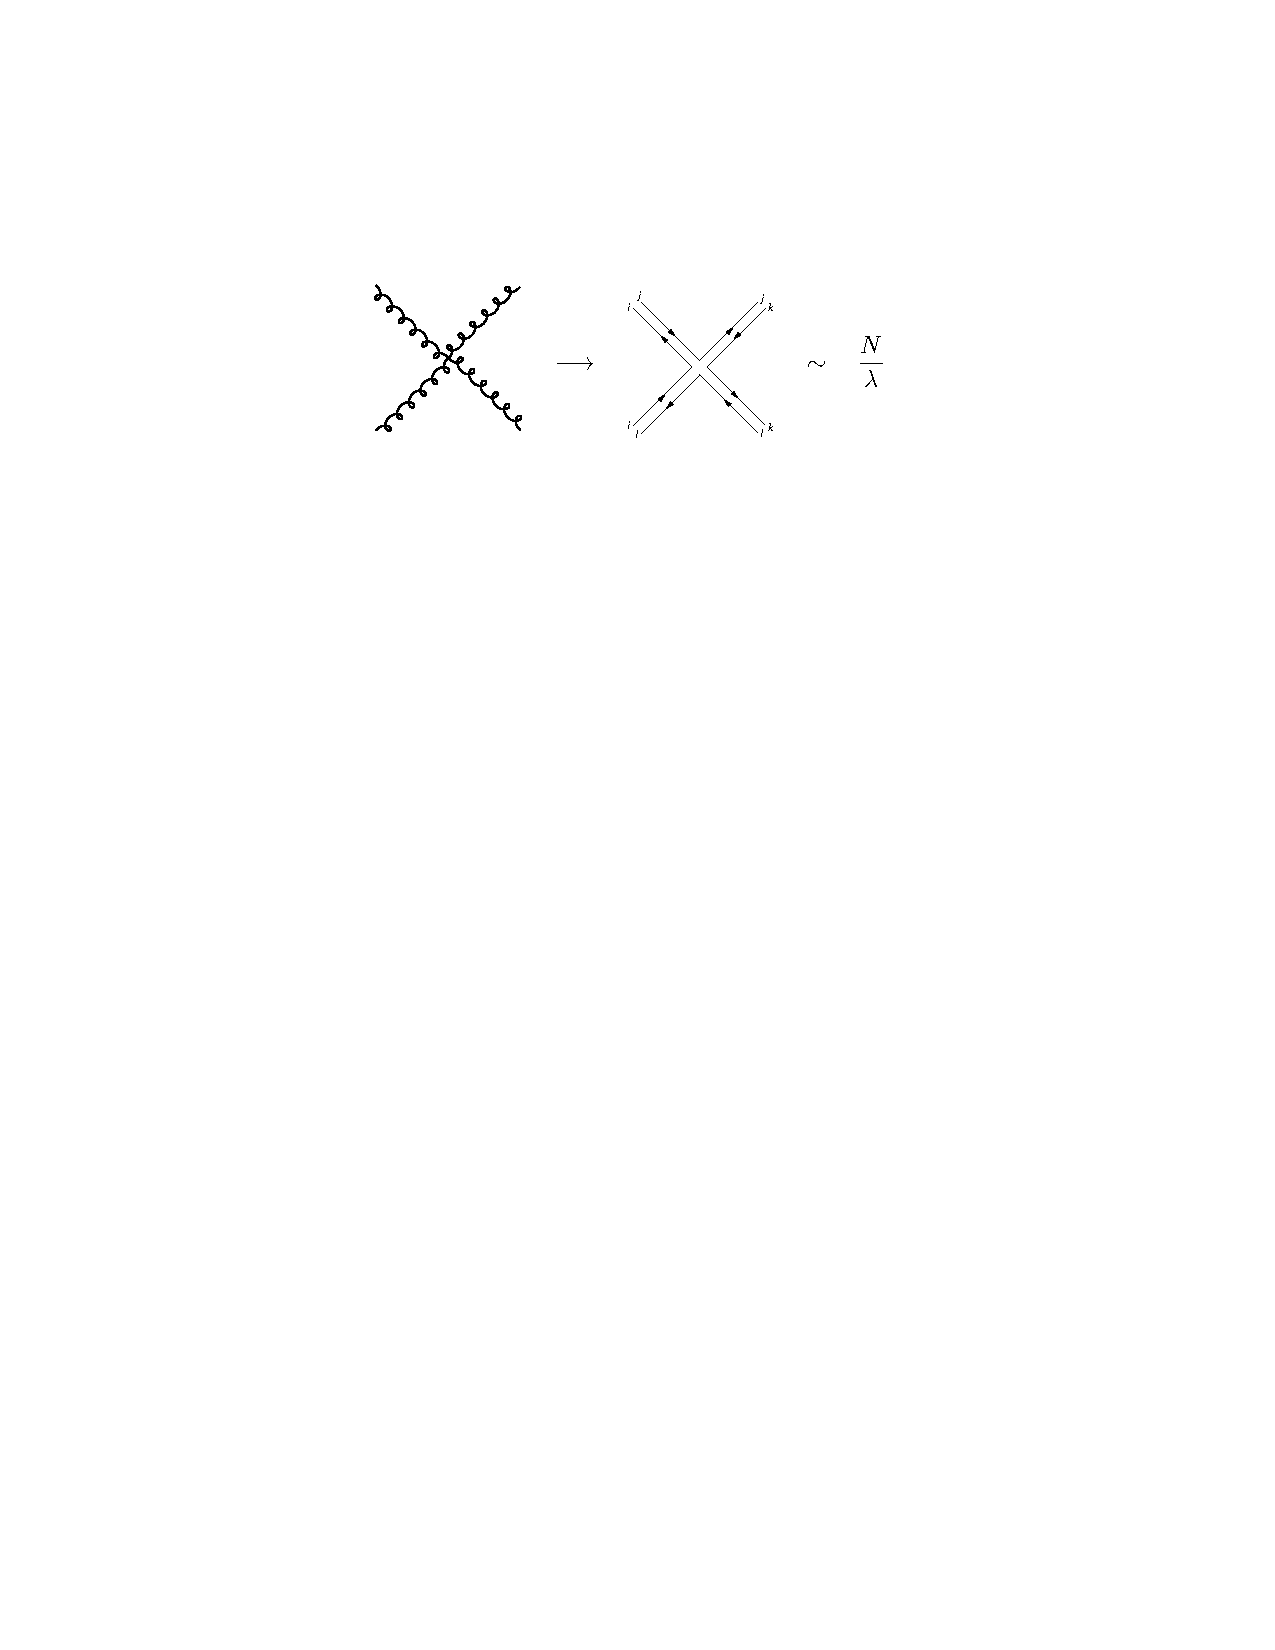
\includegraphics{figs/fig16.pdf}
\end{figure}
根据\ref{B.5}的经验,每个圈代表一个指标缩并,带来额外的$N$:
\begin{equation}
	\text{diagram}\sim\left(\frac{\lambda}{N}\right)^{\#\text{propagators}} \left( \frac { N }{ \lambda }\right)^{\#\text{vertices}}N ^ {\#\text{loops}}
\end{equation}
完整的带源的配分函数或许很难求,但是作为归一化因子的真空泡泡图研究起来还是相对简单,稍微画画就能知道不是所有的图都能在平面上画出来还没有交叉,或者说在球面上画不出来。注意二维曲面分类定理,这个定理说的是任何二维闭流形都可以用其是否可定向和Euler数来分类,费曼图肯定都是嵌入可定向的流形里面,对应的Euler数就是数这个流形有几个洞,也就是亏格$g$:\footnote{反正我学拓扑记的最深刻的就是这个极为优美的定理了,虽然表述起来只需要点集拓扑,但是最简单的证明是通过代数拓扑计算基本群得到的!}
\begin{equation}
	\chi(g)=V+F-E=2-2g
\end{equation}
而一个费曼图最少需要几个洞洞的流形来承载就告诉了我们这个图在大$N$极限下的行为:
\begin{equation}
	\mathrm{diagram}\sim N^{\chi}\lambda^{E-V}
\end{equation}
$\lambda$是一个固定的数,不用关心。比如:
\begin{figure}[H]
	\centering
	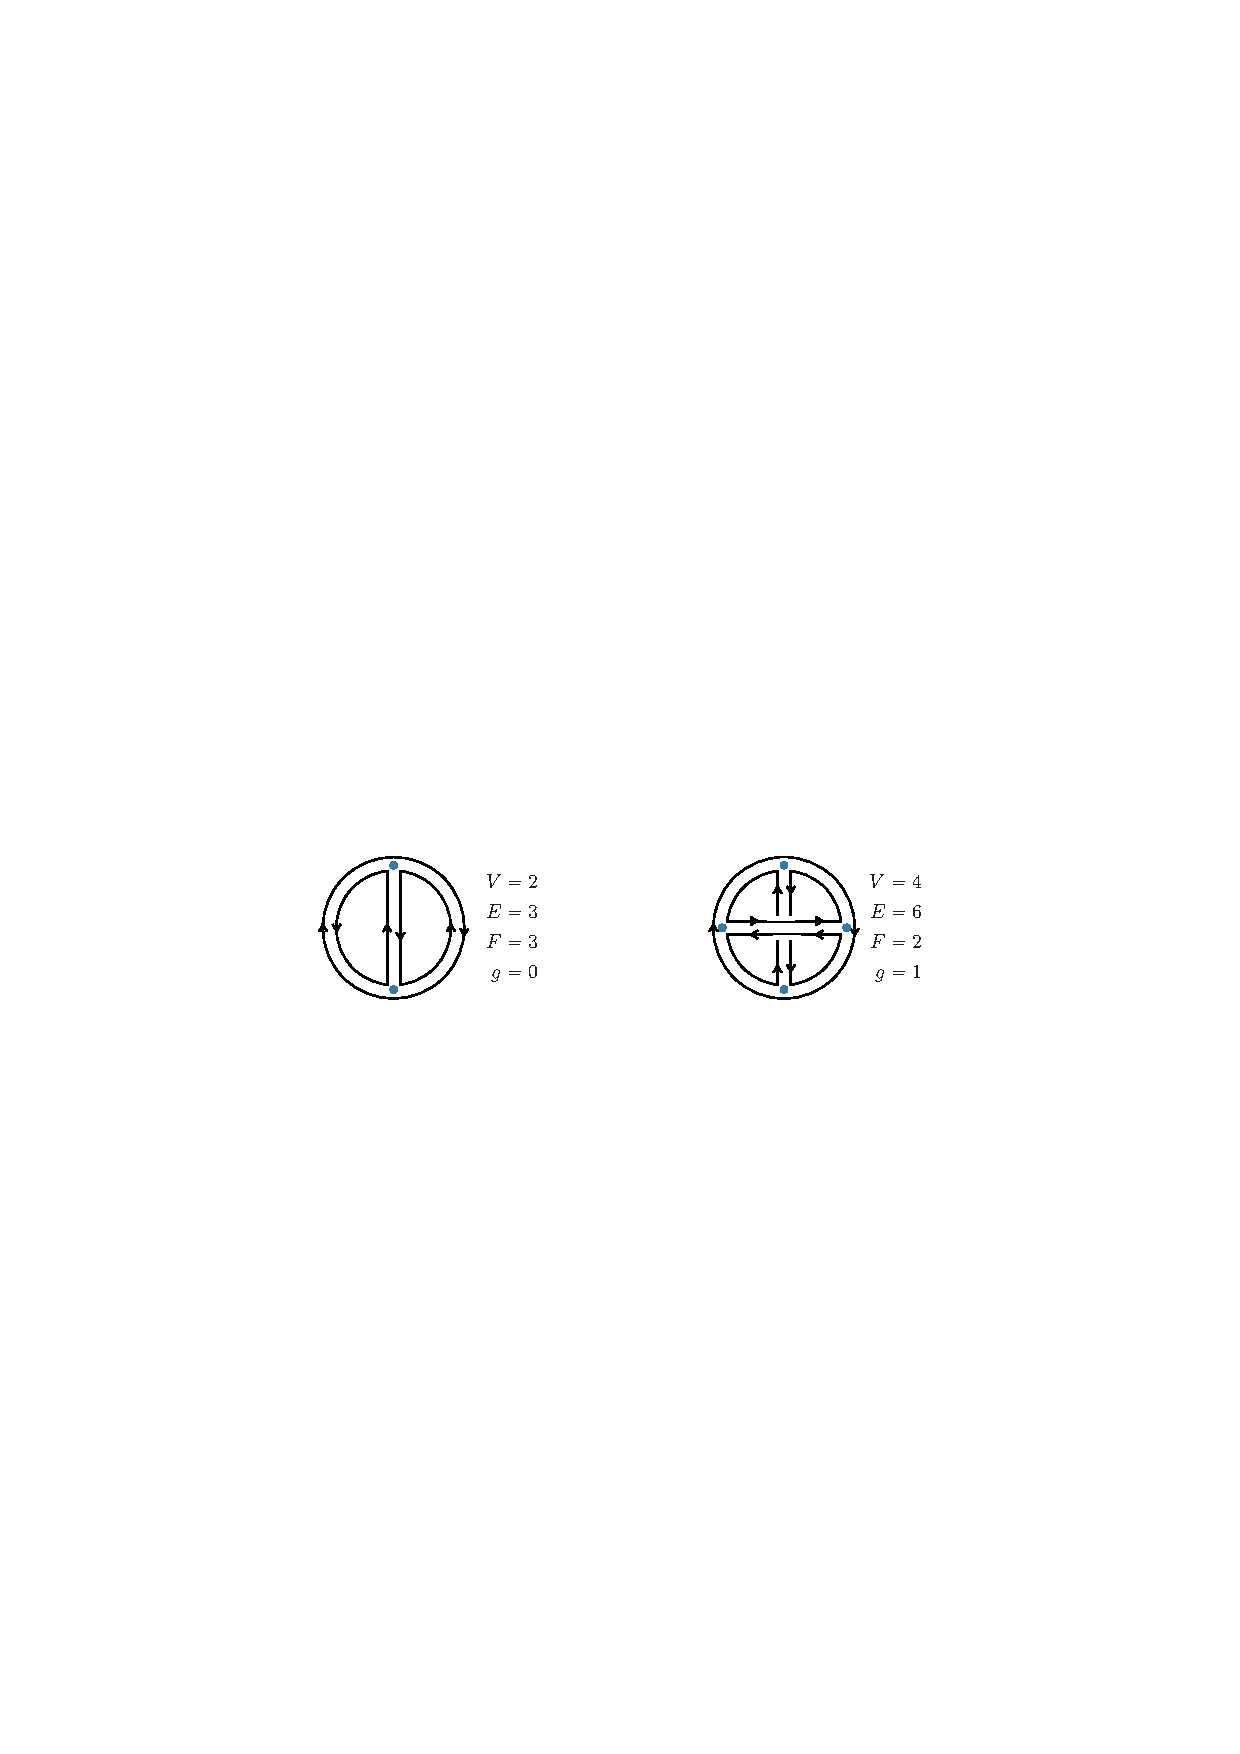
\includegraphics{figs/fig17.pdf}
\end{figure}
所以在$N\to\infty$,只有$\chi=2$的平面图有贡献。

看似这一节讲的东西和AdS/CFT没有半毛钱关系,虽然$YM$在树图阶是共形不变的,AdS呢?或者说引力在哪里?前面这一堆我们按照拓扑结构一级一级将真空图的贡献按照$N$进行展开,首先这一点就不同于通常的QFT,通常的QFT就是按照图的顶点数目进行展开,没有涉及到拓扑结构,但这一点在弦论里面非常重要,弦论结果的微扰展开就是根据拓扑结构进行展开的!比如最低阶对应的就是球面,subleading阶就是甜甜圈造型。这暗示着或许大$N$极限下的YM理论和弱耦合的弦论有某种对应(这样弦论微扰展开就只需要考虑球面那一阶)。事实确实如此:\footnote{下面式子刻画的比较粗糙,但够用。}
\begin{equation}
	N\sim g_s^{-1},\quad\alpha^{\prime}\longleftrightarrow\lambda 
\end{equation}

这里$g_s$是弦论里面的耦合常数,$\alpha^\prime$和弦上的张力有关。而弱耦合的弦论又会直接对应到Einstein引力,所以似乎可以直接从Yang-Mills理论里面得到量子引力!这是AdS/CFT最早的线索,不过即使是加入了超对称的超弦理论也得生活在$9+1$维时空,远大于$3+1$维时空,至少目前为止,没有从纯YM理论出发来建立引力对偶,毕竟对应的玻色弦要生活在26维时空,这差的就太远了。从超弦理论,已经\textbf{严格}建立起来了$AdS_{5}\times\mathcal{S}^5$的量子引力理论与$\mathcal{N}=4$的SYM理论之间的对偶,SYM理论生活在$AdS_5$的$3+1$维边界上。这也兴起了AdS/CFT研究的浪潮!不过这二十年来,唯一严格建立起来的对偶只有这一个,其它的各种对偶只是两头算出来的结果能对上,所以猜测对偶是存在的,后面要介绍的一些对偶工具也属于此类。

\subsection{大$N$极限量子色动力学}这一小节的目的就是把费米子单线加进去看看大$N$展开的形式,严格来说偏离主线。
\begin{equation}
	S_{QCD}=N\int d^4x\left(-\frac{1}{2\lambda}\mathrm{tr}F^{\mu\nu}F_{\mu\nu}+i\bar{\psi}D\psi \right)
\end{equation}
为了得到上面的作用量,对费米子做了rescale,$\psi\mapsto\sqrt{N}\psi$。需要加入下面的单线:
\begin{figure}[H]
	\centering
	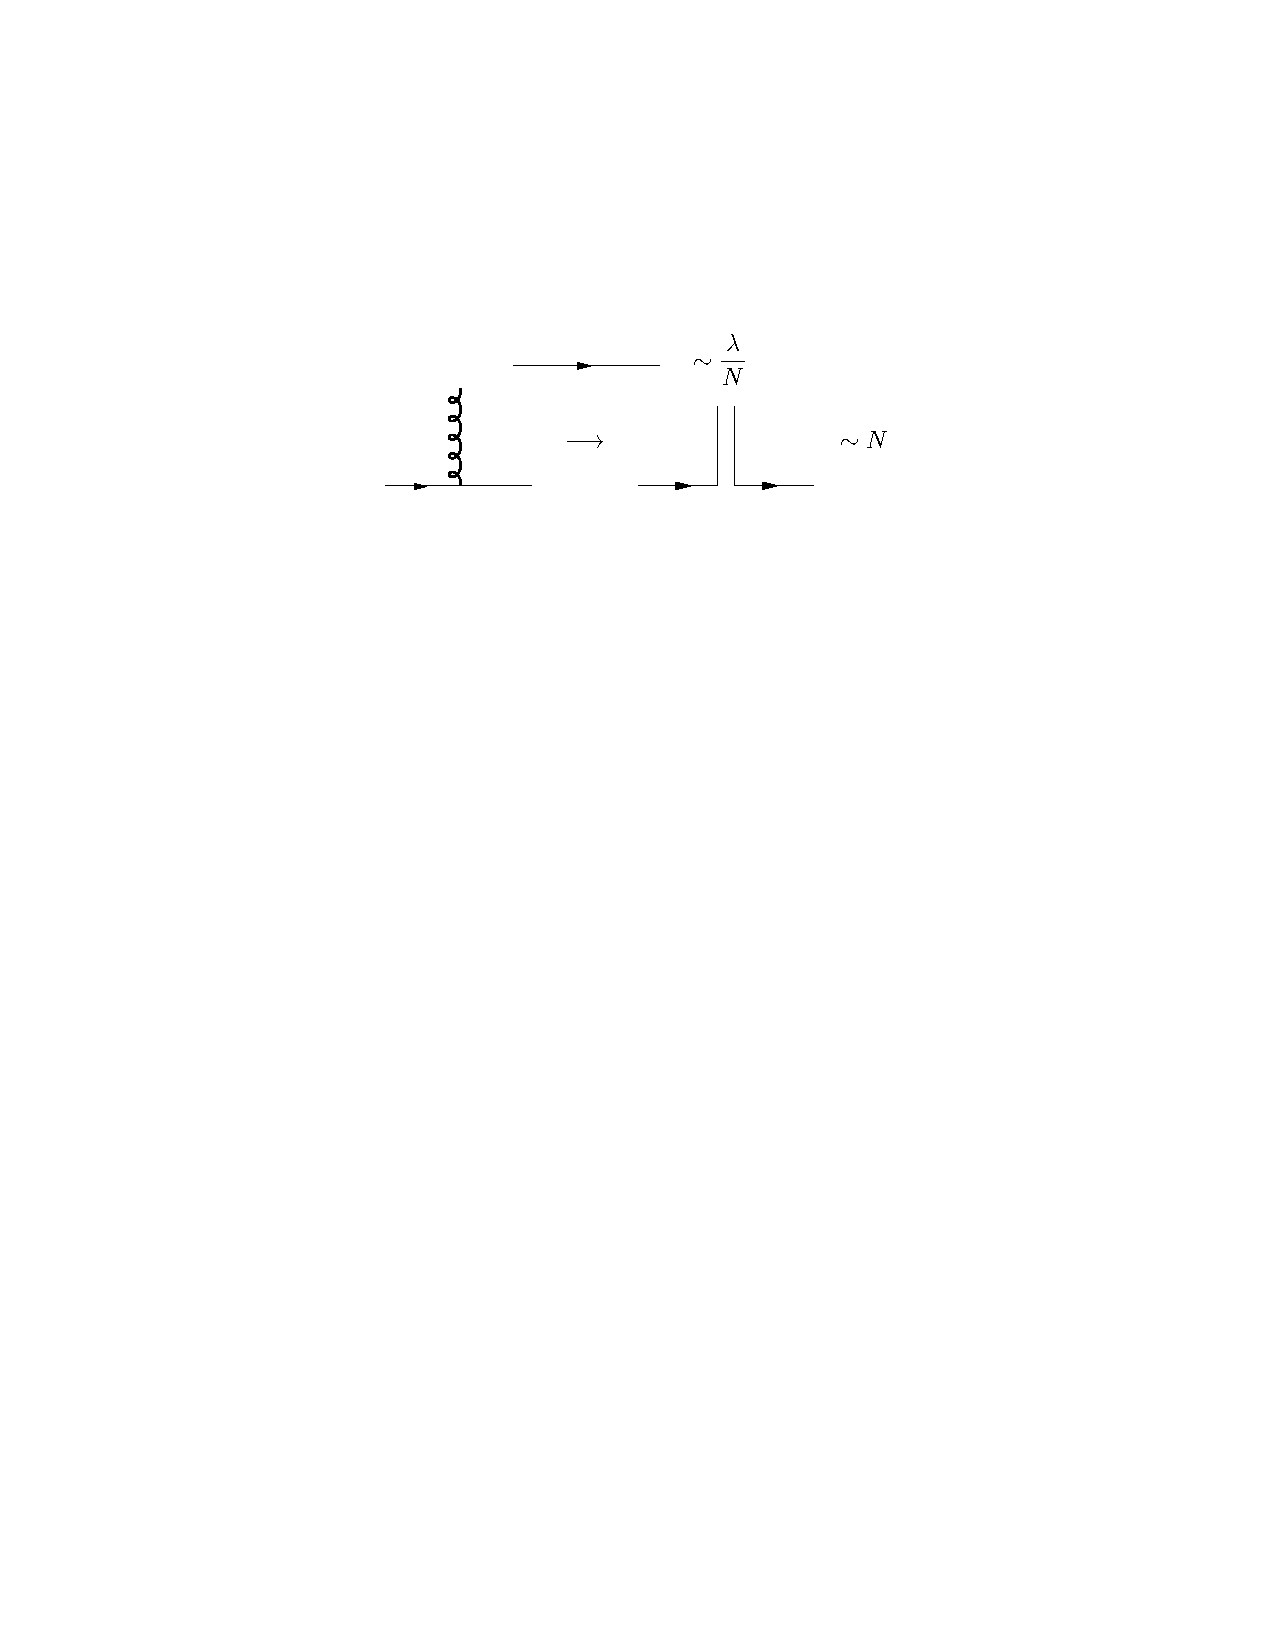
\includegraphics{figs/fig18.pdf}
\end{figure}
依然考虑真空图,依旧可以根据拓扑结构展开:
\begin{equation}
	\mathrm{diagram}\sim N^\chi\lambda^{E-V}
\end{equation}
唯一的差别是由于单线的引入,现在的费曼图不能看成是一个闭流形,而要看成一个带边流形,每个费米子线是一个边界连通分支$B$,带边(紧致)流形同样有分类定理,这个时候除了可定向性和亏格,还需要边界连通分支数目$B$,可定向带边(紧致)二维流形Euler数为:
\begin{equation}
	\chi=2-2g-B
\end{equation}
\begin{remark}
	亏格为$g$的不带边曲面$gT^2$可以看作是一个球面和$g$个甜甜圈的连通和(粘起来,然后把重叠的区域那块墙打通),而还带有$B$个边界连通分支的带边紧致曲面可以看作是在$fT^2$的基础上挖去$B$个圆盘的内部(这样圆盘的边界就剩下来了)。
\end{remark}
比如下面这个例子:

胶子介子衰变还有OZI压低,这部分还很重要,未完待续
